\section{Introduction}

Real-world software development involves large source code repositories.
Reading and trying to understand other people's code in such repositories
is a difficult and unpleasant process for many software developers,
especially when the code is not sufficiently commented.
For example, if the Java method in Fig.~\ref{figure:sourceCodeExample} does not
have the comment in the beginning, it will take the programmer
quite some efforts to grasp the meaning of the code.
However, with a meaningful sentence such as
%``Returns true when one of the rows already contains all the pairs''
``calculates dot product of two points''
as a descriptive comment, programmer's
productivity can be tremendously improved.
%\KZ{Can our algo really generate such as fancy comment?If not maybe use an example that we can generate?}

%\begin{figure}[th]
%\begin{lstlisting}
%// Returns true when one of the rows already contains all the pairs
%  private static boolean isPartialRow(Iterable<ExpandedPair> pairs, Iterable<ExpandedRow> rows) {
%    for (ExpandedRow r : rows) {
%      boolean allFound = true;
%      for (ExpandedPair p : pairs) {
%        boolean found = false;
%        for (ExpandedPair pp : r.getPairs()) {
%          if (p.equals(pp)) {
%            found = true;
%            break;
%          }
%        }
%        if (!found) {
%          allFound = false;
%          break;
%        }
%      }
%      if (allFound) {
%        return true;
%      }
%    }
%    return false;
%  }
%\end{lstlisting}
%%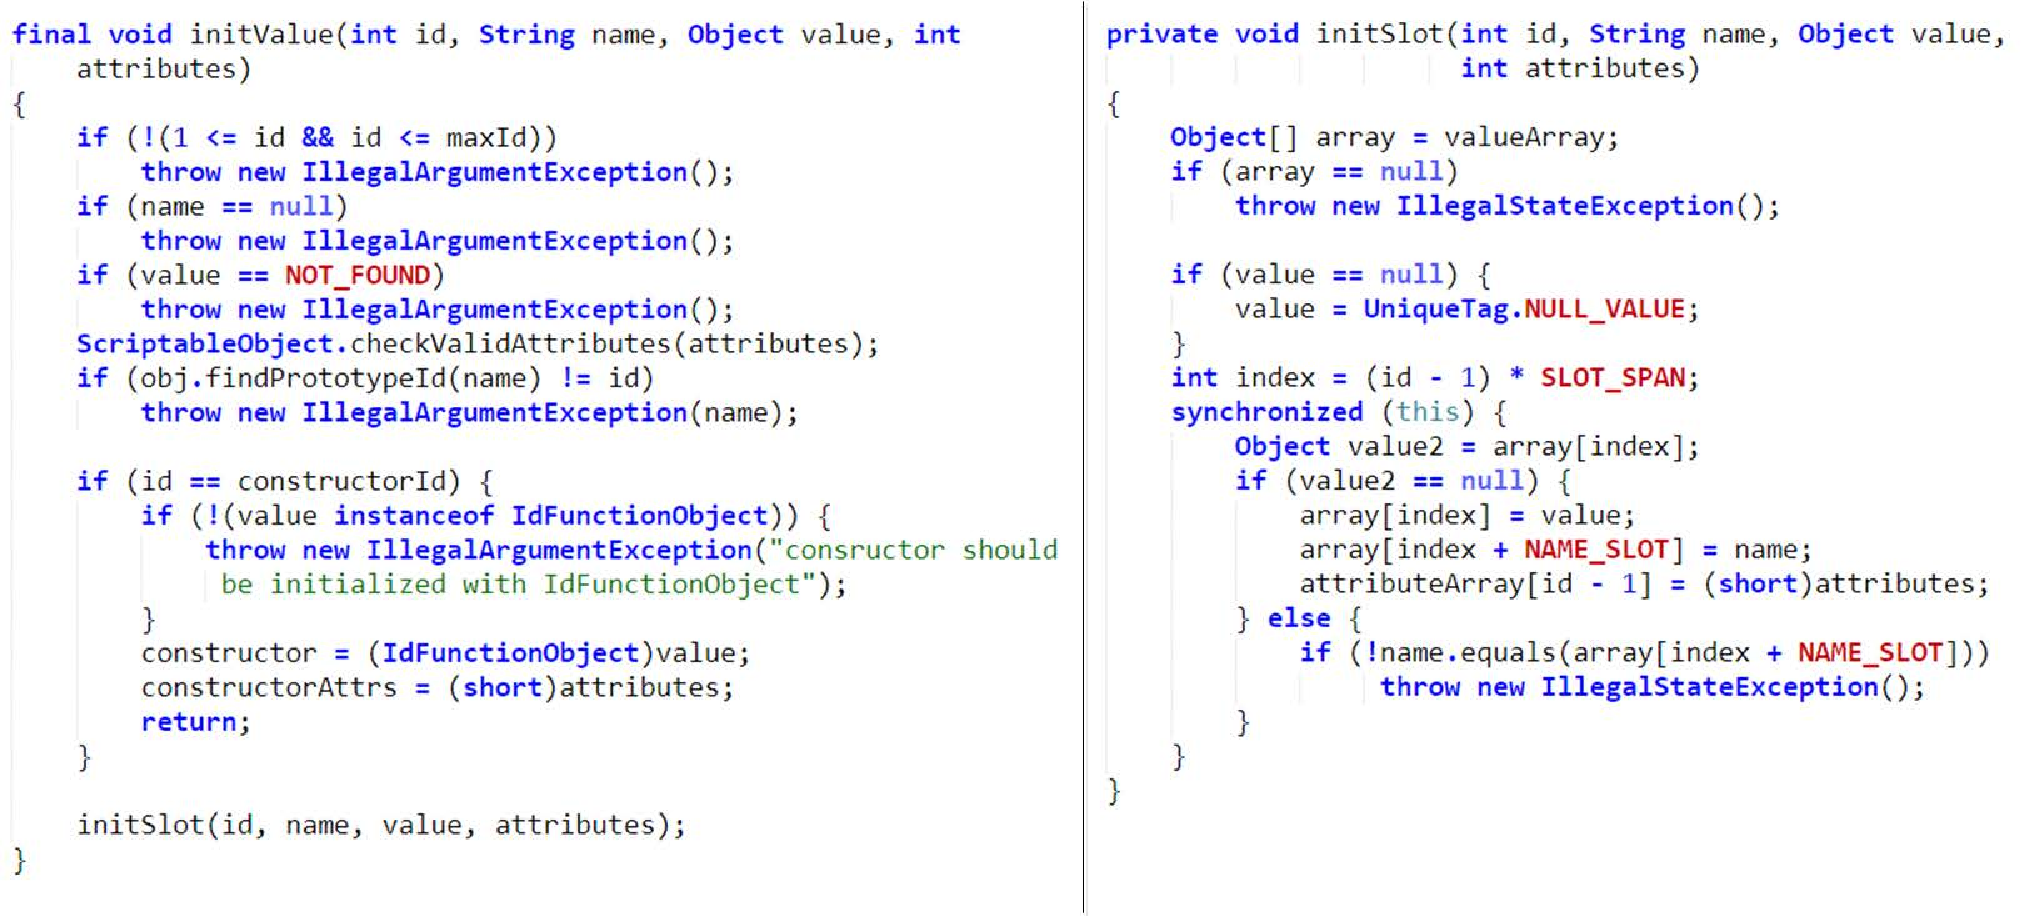
\includegraphics[width=16cm]{img/codeExample.pdf}
%\caption{\label{figure:sourceCodeExample}source code example}
%\end{figure}

\begin{figure}[th]
\begin{lstlisting}
    /* Calculates dot product of two points.
     * @return float */
    public static float ccpDot(final CGPoint v1, final CGPoint v2) {
        return v1.x * v2.x + v1.y * v2.y;
    }
\end{lstlisting}
%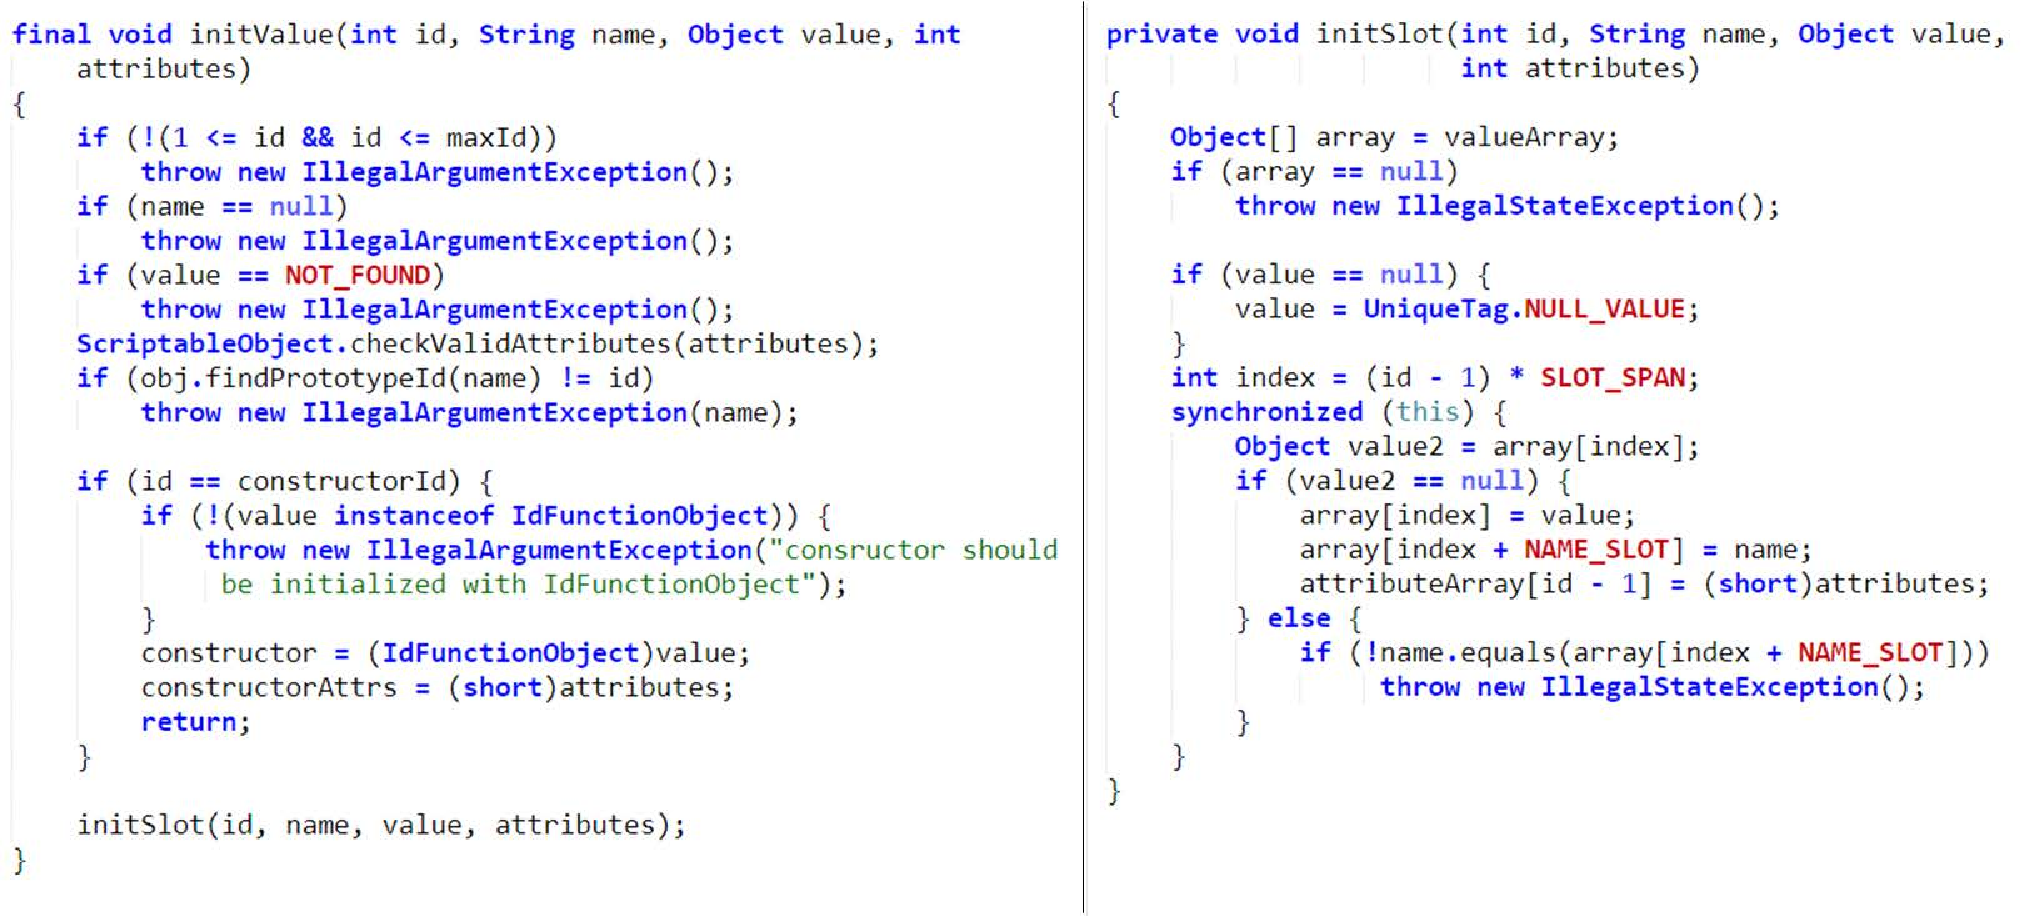
\includegraphics[width=16cm]{img/codeExample.pdf}
\caption{\label{figure:sourceCodeExample}source code example}
\end{figure}


A related scenario happens when one wants to search for a piece of code with
a specific functionality or meaning. Ordinary keyword search would not work
because expressions in programs can be quite different from natural languages.
If methods are annotated with meaningful natural language comments, then
keyword matching or even fuzzy semantic search can be achieved.

Even though comments are so useful, programmers are not using them enough in their
coding. Table \ref{table:repos} shows the number of methods in
ten actively developed Java repositories from Github, and those of
which annotated with a descriptive comment.
On average, only 15.4\% of the methods are commented.

%Finally, code pieces which look quite different on the surface, due to
%the use of different identifier names and different code structures,
%may actually serve the same purpose.
%Detecting duplicated or similar code fragments in a large repository
%is a common software engineering practice that simplifies the maintenance
%efforts and lowers development costs. Again, if all code pieces are sufficiently
%commented, similar pieces can be detected by comparing their comments.
%\KZ{Is that really necessary (to generate comments)? Maybe just obtaining the vector
%rep of the code is sufficient?}

\begin{table*}[th]
\caption{\label{table:repos} Ten Active Projects on Github}
\center
\scriptsize{
\begin{tabular}{|c|c|c|c|c|c|}
\hline
Project & Description & \# of bytes & \# of Java Files& \# of Methods& \# Methods Commented\\
\hline \hline
Activiti & a light-weight workflow and Business Process Management (BPM) Platform & 168M & 2939 & 15875 & 1080 \\
\hline
aima-java & Java implementation of algorithms from ``Artificial Intelligence - A Modern Approach'' & 182M & 889 & 4078 & 1130\\
\hline
neo4j & the world��s leading Graph Database. & 270M & 4125 & 24529 & 1197 \\
\hline
cocos2d & cocos2d for android, based on cocos2d-android-0.82 & 78M & 512 & 3677 & 1182 \\
\hline
rhino & a Java implementation of JavaScript.& 21M & 352 & 4610 & 1195 \\
\hline
spring-batch & a framework for writing offline and batch applications using Spring and Java & 56M & 1742 & 7936 & 1827 \\
\hline
Smack & an open source, highly modular, easy to use, XMPP client library written in Java & 41M & 1335 & 5034 & 2344\\
\hline
guava & Java-based projects: collections, caching, primitives & 80M & 1710 & 20321 & 3079 \\
\hline
jersey & a REST framework that provides JAX-RS Reference Implementation and more. & 73M & 2743 & 14374 & 2540\\
\hline
libgdx & a cross-platform Java game development framework based on OpenGL (ES)& 989M & 1906 & 18889 & 2828 \\
\hline
\end{tabular}

\begin{tablenotes}
 \item[1] A comment here refers to the description at the beginning
of a method, with more than eight words.
\end{tablenotes}
}
\end{table*}

To automatically generate descriptive comments from source code,
one needs a way of accurately representing the semantics of code blocks.
One potential solution is to treat each code block as a document
and represent it by a topic distribution using models such as LDA~\cite{blei2003latent}.
However, topic models, when applied to source code,
have several limitations:

\begin{itemize}
\item a topic model treats documents as a bag of words and ignores the
structural information such as programming language syntax and
function or method calls in the code;
\item the contribution of lexical semantics to the meaning of code
is exaggerated;
\item comments produced can only be words but not phrases or sentences.
\end{itemize}

%\KZ{One step toward making the generated comments more readible is to
%use templates to generate comments \cite{}. Give some descriptions of
%such approach and its limitations. Give examples here to show why they
%are not good enough.}
%
%\KZ{State the challenges in our problem.}

One step toward generating readable comments is to
use templates~\cite{mcburney2014automatic,sridhara2010towards}.
The disadvantage is that comments created by templates are often
very similar to each other and only relevant to parts of the code
that fit the template.
For example, the comment generated by McBurney's model
for Fig.~\ref{figure:sourceCodeExample} is fairly useless:
%\noindent\fbox{
%\parbox{\columnwidth}{
{\em ``This method handles the ccp dot and returns a float.
ccpDot() seems less important than average because it
is not called by any methods.''
}


To overcome these problems,
%we have to find a meaningful method to represent the source code first, then decode these representation into meaningful comments.
in this paper, we propose to use Recursive Neural Network
(RNN)~\cite{socher2011parsing,socher2011semi} to
combine the semantic and structural information from code.
%Recursive Neural Network has been used in NLP field before, such as by
%Socher et al.~ and by
%Irsoy and Cardie~\cite{irsoy2014deep}.
Recursive NN has previously been applied to parse trees of natural language sentences, such
as the example of two sentences in Fig.~\ref{rnn:nlp}.
In our problem, source codes can be
accurately parsed into their parse trees, so recursive NN can be applied
in our work readily. To this end, we design a new recursive NN called
Code-RNN to extract the features from the source code.

\begin{figure}[th]
	\centering
	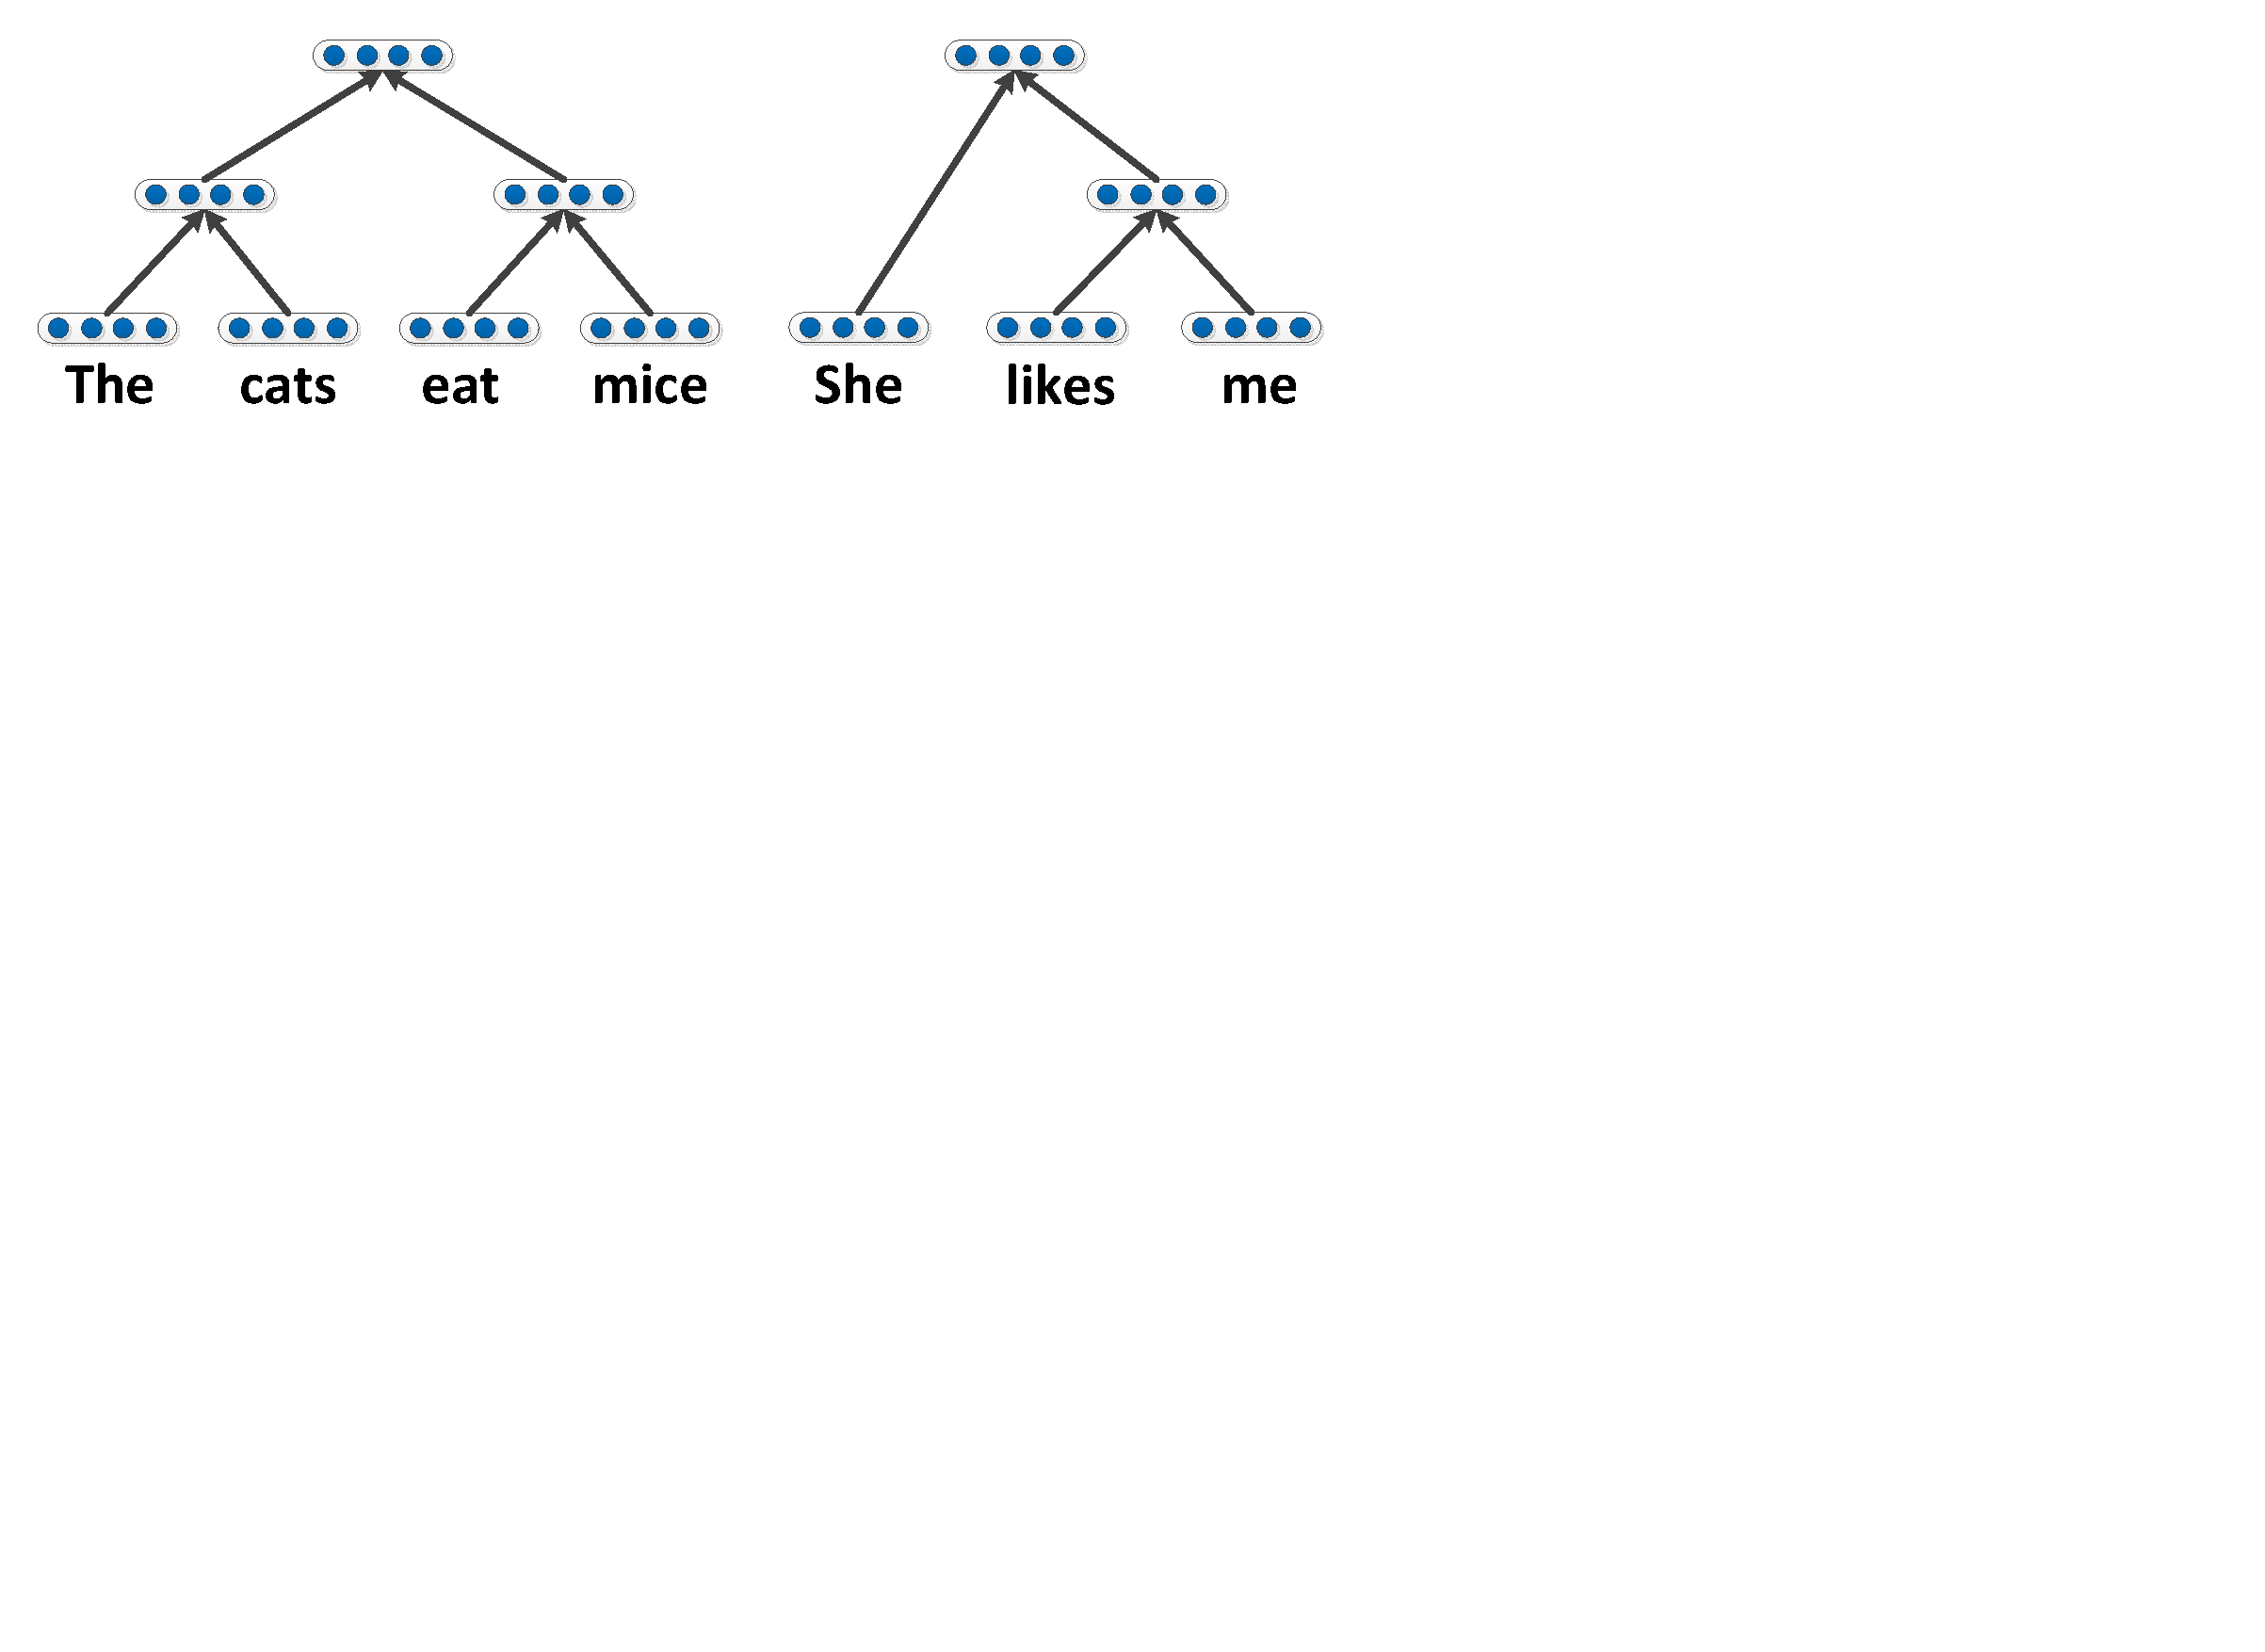
\includegraphics[width=\linewidth]{img/rnn_1.pdf}
	% where an .eps filename suffix will be assumed under latex,
	% and a .pdf suffix will be assumed for pdflatex; or what has been declared
	% via \DeclareGraphicsExtensions.
	\caption{The Recursive Neural Networks of Two Sentences}
	\label{rnn:nlp}
\end{figure}

%The parse trees in natural language process are all binary trees \KZ{This is
%not true, dependency parse is not binary...}
%but the trees in source code are arbitrarily trees, so we design a new Recursive Neural Network called Code-RNN to extract the information of source code.

Using Code-RNN to train from the source code, we can get
a vector representation of each code block and this vector contains
rich semantics of the code block, just like word
vectors~\cite{mikolov2013distributed}. We then use a Recurrent Neural
Network to learn to generate meaningful comments.
Existing recurrent NN %(\KZ{What kind of RNN})
does not take good advantage of the code block representation vectors.
Thus we propose a new GRU~\cite{cho2014properties} cell that does a better job.

In sum, this paper makes the following contributions:
\begin{itemize}
\item by designing a new Recursive Neural Network, \emph{Code-RNN},
we are able to describe the {\em structural information} of source code;
\item with the new design of a GRU cell, namely \emph{Code-GRU}, we make the best
out of code block representation vector to effectively generate comments
for source codes;
\item the overall framework achieves remarkable accuracy (Rouge-2 value) in the task of
generating descriptive comments for Java methods,
compared to state-of-the-art approaches.
%\item by adding method invocation information to the model,
%we strengthen the ability to generate comments for other methods who have no manual comments;
%\item by splitting one parse tree into many subtrees, we make the Code-RNN has the same depth for all methods.
\end{itemize}

%Next, we first present our approach, as well as some evaluation results, then
%discuss some related work before concluding the paper.
